\begin{frame}{Problemstellung}

\begin{itemize}
	\item Barrier-Bucket System \uncover<2-> {: 
		\begin{itemize}
			\item Longitudinale Manipulation der Bunches
		\end{itemize}
		}
	\item \uncover<3-> { Ziel } \uncover<4->{:
		\begin{itemize}
			\item Gap Spannung in Form einer Ein-Sinus Periode
			\item Qualität das Signals
		\end{itemize}
		}
		
		%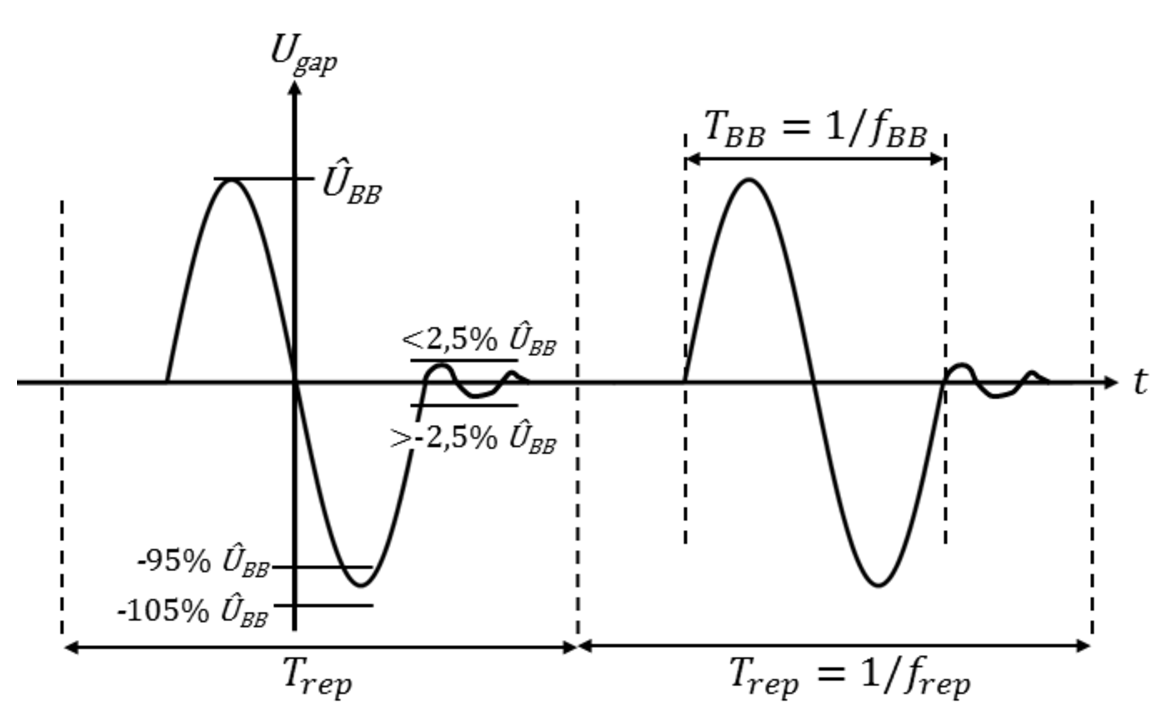
\includegraphics[scale=0.3]{slides/Problemstellung/BB_req.eps}
\end{itemize}		
\uncover<4-> {		
	\begin{picture}(10,7)
		\put(70,-90){
			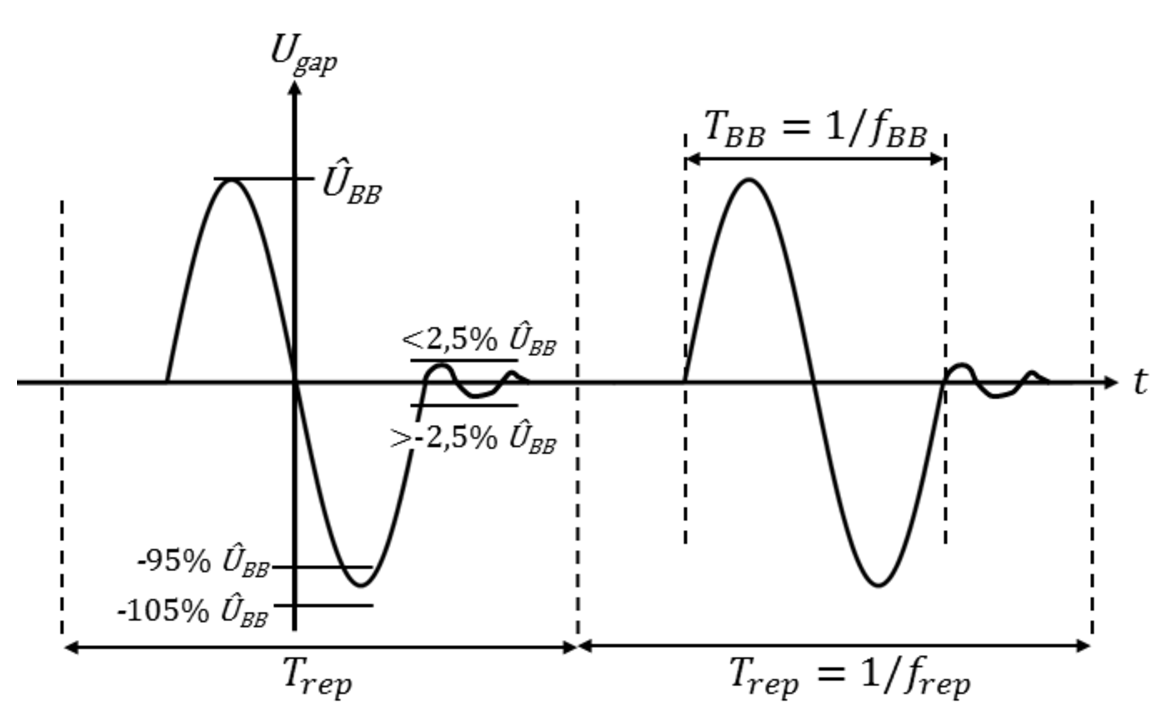
\includegraphics[scale=0.3]{slides/Problemstellung/BB_req.eps} 
		}  
	\end{picture} 
}	

\end{frame}



